\documentclass[12pt]{ctexart}%中文包
\usepackage{graphicx}%图片引用包
\usepackage{amssymb}%特殊符号
\usepackage{amsmath,amsfonts,bm}%矩阵
\usepackage{amsthm}%定理
\usepackage{geometry}%缩放
\usepackage{hyperref}%超链接
\usepackage{framed}%框框
\usepackage{color}%颜色
\usepackage{mathrsfs}%花体
\usepackage{anyfontsize}
\usepackage{indentfirst}%缩进
\usepackage{extsizes}%size
\usepackage{newtxtext,newtxmath}%times风格字体
\usepackage{mdframed}%边栏

\surroundwithmdframed[
  linecolor=gray,
  topline=false,
  bottomline=false,
  rightline=false,
  linewidth=4pt,
  innerleftmargin=10pt,
  innerrightmargin=10pt,
  innertopmargin=0pt,
  innerbottommargin=5pt
]{theorem}
\newtheorem{theorem}{Law}
\geometry{a4paper,scale=0.85}
\hypersetup
    {
        hypertex=true,
        colorlinks=true,
        linkcolor=blue,
        anchorcolor=blue,
        citecolor=blue
    }

\title{Wave Function and Light\\波函数和光}

\author{Jerry Ling} 

\date{\today}
 
\begin{document}  %begin后括号内是文件类型
\maketitle  %生成标题
在量子化学中,我们认识到光的波粒二象性。对光学现象的理解因而也有若干层面,即几何光学、物理光学和量子光学。因为光作为一种电磁波已经被研究地较为透彻,我们不妨选取中间的途径,从波动现象构建知识体系。本章重点关注从普遍的波动现象抽象出一维的波动方程,并引出其满足微分方程。

\section*{非色散(non-dispersive)波动方程导出}
考虑一根二维平面上的绳子并上下摆动之。由于绳子材质的张力这种振动会沿着绳子的方向传播。我们将某种运动模式的传播过程成为波(wave)。设改振动模式在空间上某点x的振动状态可以用$\psi(x)$来描述。因为波随着时间变化,所以它也是时间的函数。那么在没有衰减(非色散,即波形不变)的一维情况下,可以预计经过时间t后该点的振动状态应以$v$的速度出现在$vt$处。即:
\begin{equation}
    \psi(x,0)=\psi(x+vt,t)
\end{equation}
用$f(x)$表示$\psi(x,0)$的具体形式,$\psi(x,t)$可写出通式:
\begin{equation*}
    f(x)=\psi(x+vt,t)
\end{equation*}
\begin{equation}
    \psi(x,t)=f(x-vt)\label{1d_wave_eq}
\end{equation}
给定初始波形,由式(\ref{1d_wave_eq})可直接写出正向的一维波动方程,反向传播需要调换正负号。或用$F(t)$表示0点振动随时间的变化,波动方程可等价地表示为:
\begin{equation}
    \psi(x,t)=F(t-\frac{x}{v})\label{1d_wave_eq2}
\end{equation}
对式(\ref{1d_wave_eq})两边分别求t和x的偏导数和二阶偏导:
\begin{equation}
    \partial_{x} \psi=f^{'}(x-vt)
\end{equation}
\begin{equation}
    \partial_{t}\psi=-v f^{'}(x-vt)
\end{equation}
\begin{equation}
    \partial^2_{xx}\psi=f^{''}(x-vt)\label{pxx}
\end{equation}
\begin{equation}
    \partial^2_{tt}\psi=v^2f^{''}(x-vt)\label{ptt}
\end{equation}
由(\ref{pxx}),(\ref{ptt})得到一维微分波动方程(one-dimensional differential wave equation):
\begin{framed}
    \begin{equation}   
        \frac{1}{v^2}\partial^2_{tt}\psi=\partial^2_{xx}\psi 
        \label{we1}
    \end{equation}
\end{framed}
注意,一维中的波形不变性不一定能推广到所有波动现象,即还存在色散波。事实上,给定波动方程, 根据微分方程的理论,对波动方程的必然解简谐波,我们可以导出波数和频率的色散关系。为了说明其中的关系,需要先考察简谐波:

\section*{简谐波,叠加和表示}
简谐波是一类性质被彻底理解的波类,是研究复杂波动现象的基础。其普遍形式见式(\ref{sin})。其中$k$为波数或空间频率,$\omega$为角频率。进一步考察发现sin括号内的成份决定了某点状态,一般称其为相(phase),记作$\varphi$:
\begin{equation}
    \varphi=kx-\omega t
\end{equation}

\begin{framed}
\begin{equation}
    \psi(x,t)=A\sin(kx-\omega t)
    \label{sin}
\end{equation}
\end{framed}
对一个\textbf{线性微分方程}(其中p表示一个关于算子的多项式):
\begin{equation}
    p(\partial_x,\partial_t)f=0
    \label{lpde}
\end{equation}
我们有两个非常好的性质。第一,解构成一个线性空间(注意,极大的振幅可能引起介质的非线性振动,应另作讨论),任意两个解的线性组合仍旧是解。第二,基本简谐波总是其特殊解。鉴于三角函数和复指数的关系和可叠加性,可以用复指数表达简谐波,两个正弦波的叠加可以直接用其\textbf{phasor}(图\ref{phasor})的矢量和导出。但需注意,对复数表示的波只能使用实数乘法的操作,不然必须转化为余弦/正弦表示。
\begin{equation}
    \psi(x,t)=Ae^{i(kx-\omega t+\epsilon)}=Ae^{i\varphi}
    \label{complex_form}
\end{equation}
一般而言,\textbf{振幅相近}的两个正弦波的叠加,根据相位差可分为in-phase和out-phase。后者倾向于削减彼此幅度的现象称之为\textbf{干涉(interference)}。这一点可通过矢量图直观理解。
\par 根据上述两点性质,对任何能展开为简谐波线性组合的初始条件$\psi(x,0)$,仍旧可以用t时刻简谐波的组合来表示波的传播。对于波形变化对波动方程,将简谐波(\ref{complex_form})代入(\ref{lpde})可得到\textbf{色散方程(dispersive equation)}:
\begin{framed}
    \begin{equation}
        p(ik,-i\omega)=0
        \label{dispersive_equation}
    \end{equation}
\end{framed}

\section*{色散和复数的进一步讨论}
将一维波动方程(\ref{we1})代入式(\ref{dispersive_equation})可以得到色散关系$\omega/k=v$。其中左边是某频率简谐波的相速度,右边是一个常数,即相速度同频率无关。考虑有色散的非相对论薛定谔方程:
\begin{equation}
    i\hbar\partial_t\psi=-\frac{\hbar^2}{2m}\partial_x^2\psi+V(x)\psi
\end{equation}
代入色散方程得到:
\begin{equation}
    \hbar\omega=\frac{(\hbar k)^2}{2m}+V(x)
\end{equation}
注意其色散方程中速度有\textbf{频率依赖性}。根据Planck和de Broglie关系该式子等价于$E=\frac{1}{2}mv^2+V(x)$,即牛顿定律的量子力学表示。
\par 色散方程可能给出复数的波数$\k=k_1+ik_2$。代入简谐波通式(\ref{complex_form}):
\begin{equation}
    \psi(x,t)=Ae^{ik_1x-i\omega t}e^{-k_2x}
\end{equation}
注意到,波数的虚部在空间上引入了一个指数衰减,称为\textbf{衰减波(attenuated wave)}。如果k为纯虚数,那么波在x方向没有传播速度,但依然在时间轴方向以$\omega$振荡,称为\textbf{隐矢波(evanescent wave)}。

\section*{平面波}
为了描述\textbf{空间}中振荡形式的延展,我们引入\textbf{波前(wavefront)}的概念。在三维空间中,波前是一个同相位的面(surface)。现实中的波前极其复杂,但我们仅需考虑几种典型的理想化波前。其中最简单的形式即平面波——一种波前为平面并垂直于转播方向的理想波。为了描述其位置,用$\vec{r}$表示位矢。若波前通过一点为$\vec{r_0}$,那么平面波波前可用如下方程描述:
\begin{equation}
    (\vec{r}-\vec{r_0})\cdot\vec{k}=0
\end{equation}
\begin{equation}
    \vec{r}\cdot\vec{k}=a
\end{equation}
\par 注意到当$\vec{k}$限定后,a唯一确定了波面位置。于是容易构建正弦调制的波前,直接将上式作为相位代入(\ref{complex_form}):
\begin{equation}
    \psi(\vec{r})=e^{i\vec{r}\cdot\vec{k}}
    \label{complex_planewave}
\end{equation}
应当将简谐平面波想象为一束无限粗、无线密、同相位的正弦波的集合,如图\ref{plane_wave}。当它们同振幅时,称为\textbf{同质的(homogeneus)}平面波。
\begin{figure}
    \begin{minipage}{0.6\linewidth}
        \centering
        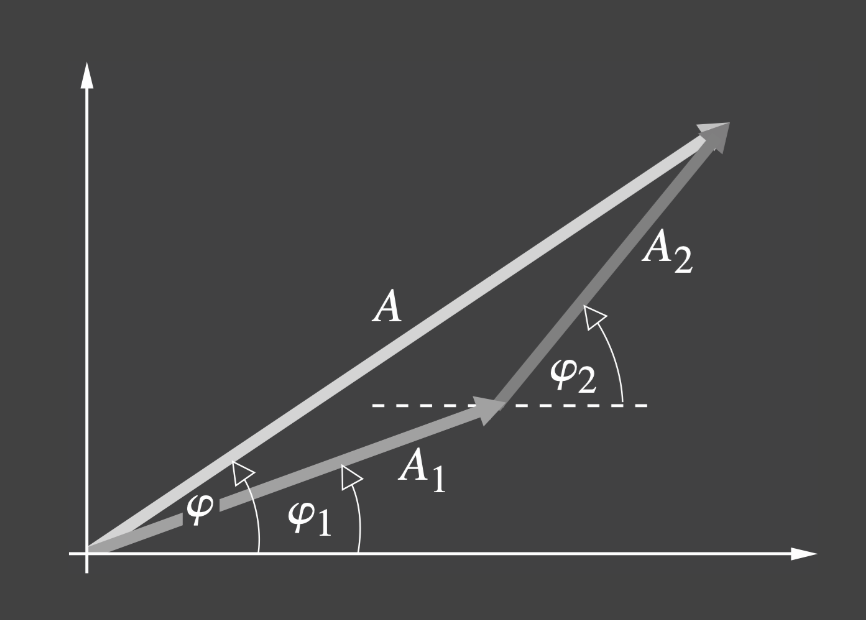
\includegraphics[width=0.8\textwidth]{Image/1_phasor.png}
        \caption{Phasor}
        \label{phasor}
    \end{minipage}
    \begin{minipage}{0.4\linewidth}
        \centering
        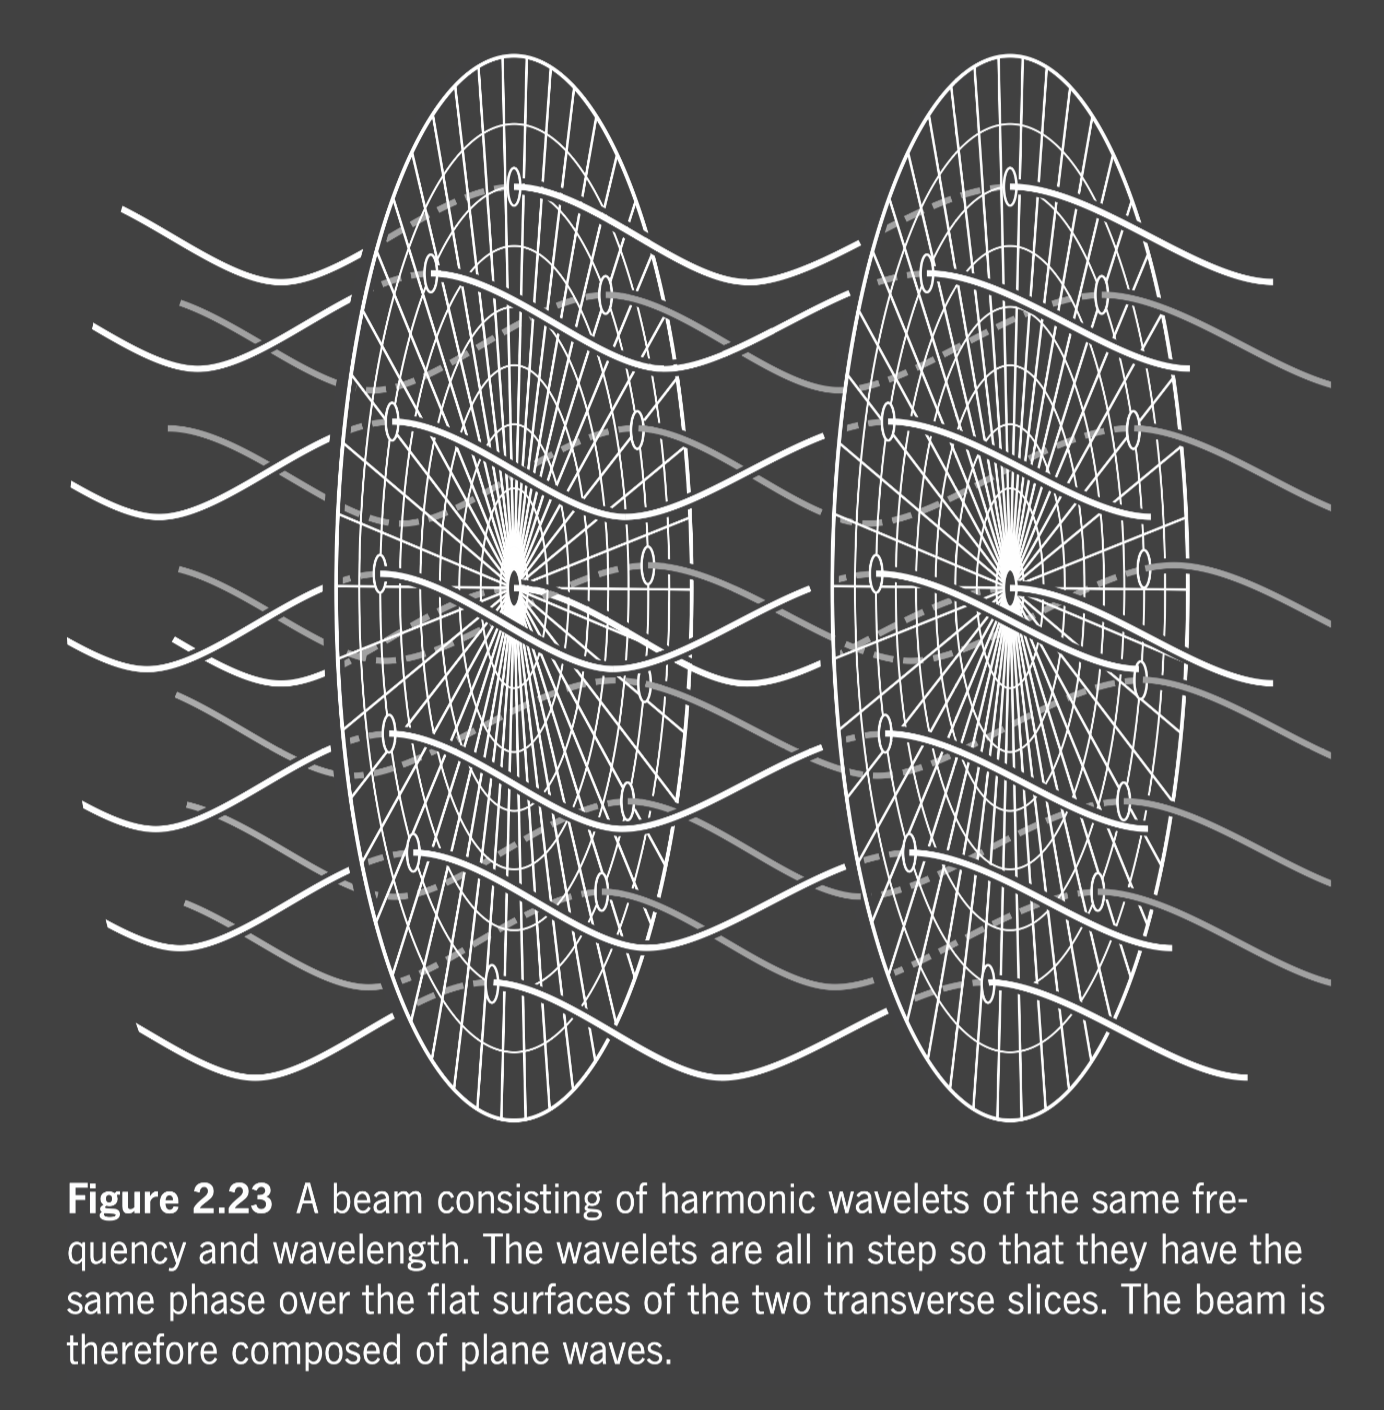
\includegraphics[width=0.85\textwidth]{Image/1_plane_wave.png}
        \caption{Visualization of plane wave}
        \label{plane_wave}
    \end{minipage}
   
\end{figure}
其空间周期$\lambda$可类似一维波地定义为$\vec{k}$方向的最小周期:
\begin{equation}
    \psi(\vec{r})=\psi(\vec{r}+\lambda \frac{\vec{k}}{k})
\end{equation}
代入(\ref{complex_planewave}):
\begin{equation}
    e^{i\vec{r}\cdot\vec{k}}=e^{i((\vec{r}+\lambda \frac{\vec{k}}{k})\cdot\vec{k})}=e^{i\vec{r}\cdot\vec{k}+i\lambda k}
\end{equation}
\begin{equation}
    \lambda=\frac{2\pi}{k}
\end{equation}
$\vec{k}$也称为\textbf{波矢(propagation vector)}。为相位引入时间变化并令相位变化速率为角速度$\omega$,得到简谐平面波的普通形式:
\begin{framed}
    \begin{equation}
        \psi(\vec{r},t)=e^{i(\vec{r}\cdot\vec{k}-\omega t)}
        \label{complex_planewave_2}
    \end{equation}
\end{framed}
\par 通过矢量$\vec{k}$我们描述了同方向的一系列平面,而通过将其放入简谐波的相位中我们建立了任意时刻的wavefront都是平面的简谐波形式。这类简谐平面波十分重要,一来因为其在实验上容易生成,二来其理论上可叠加出任意三维空间中的波。下面我们考虑三维空间中普遍的波动方程形式。

\section*{三维微分波动方程及其解}
由(\ref{complex_planewave_2})得到分量形式:
\begin{equation}
    \psi(x,y,z,t)=\exp(ik(x\alpha+y\beta+z\gamma)-i\omega t)
\end{equation}
该式必然是三维微分方程的特解,故类比(\ref{we1})导出方式,对三个坐标分量和时间分别取二次微分:
\begin{equation}
    \partial^2_{xx}\psi=-k^2\alpha^2\psi
\end{equation}
\begin{equation}
    \partial^2_{yy}\psi=-k^2\beta^2\psi
\end{equation}
\begin{equation}
    \partial^2_{zz}\psi=-k^2\gamma^2\psi
\end{equation}
\begin{equation}
    \partial^2_{tt}\psi=-\omega^2\psi
\end{equation}
结合四个式子,利用三个角度平方和为1和$\omega-k-v$关系,得到\textbf{三维波动方程}:
\begin{framed}
    \begin{equation}
        \partial^2_{xx}\psi+\partial^2_{yy}\psi+\partial^2_{zz}\psi=\nabla^2\psi=\frac{1}{v^2}\partial^2_{tt}\psi
    \end{equation}
\end{framed}
\par 对平面波而言,利用笛卡尔坐标容易导出以下两个通解:
\begin{equation}
    \psi(x,y,z,t)=f(x\alpha+y\beta+z\gamma-vt)
\end{equation}
\begin{equation}
    \psi(x,y,z,t)=g(x\alpha+y\beta+z\gamma+vt)
\end{equation}
其线性组合显然也是波动方程的解。而对于具有其他对称性的理想波而言,使用特殊的坐标系是更自然的。考虑波前为等半径球面的\textbf{球面波(spherical wave)},则定态波函数只和半径有关,使用球坐标下的算子可大幅简化微分方程:(Form given in (\ref{laplace_sph}))
\begin{equation}
    \psi(\vec{r},t)=\psi(r,t)
\end{equation}
\begin{equation}
    \nabla^{2}= \frac{1}{r^{2}} \frac{\partial}{\partial r}\left(r^{2} \frac{\partial}{\partial r}\right)+\frac{1}{r^{2} \sin \theta} \frac{\partial}{\partial \theta}\left(\sin \theta \frac{\partial}{\partial \theta}\right)+\frac{1}{r^{2} \sin ^{2} \theta} \frac{\partial^{2}}{\partial \phi^{2}}
    \label{laplace_sph}
\end{equation}
\begin{equation}
    \nabla^2\psi=\frac{1}{r}\partial^2_{rr}(r\psi)
\end{equation}
\begin{equation}
    \partial^2_{rr}(r\psi)=\frac{1}{v^2}\partial^2_{tt}(r\psi)
    \label{dwe_sph}
\end{equation}
由式(\ref{dwe_sph})容易解出球面波函数的通解:
\begin{equation}
    \psi(r,t)=\frac{f(r-vt)}{r}
\end{equation}
\begin{equation}
    \psi(r,t)=\frac{g(r+vt)}{r}
\end{equation}
简谐函数作为f或g得到\textbf{简谐球面波(harmonic spherical wave)}:
\begin{framed}
    \begin{equation}
        \psi(r,t)=\left(\frac{\mathscr{A}}{r}\right)\cos{k(r\mp vt)}
    \end{equation}
\end{framed}
其中$\mathscr{A}$称为\textbf{源强度(source strength)},波的“强度”随半径呈一次反比的衰减。符号取正的波函数为收敛波,仅存在于理想情况。
\par 另一种对称性源于圆柱体,振动源为一根无限长的线,其形成的波称为\textbf{圆柱波(cylindrical wave)},实验上可以用平面波+狭长窄缝(slit)生成。拉普拉斯算子和微分方程有如下化简形式:
\begin{equation}
    \nabla^{2}= \frac{1}{r} \frac{\partial}{\partial r}\left(r \frac{\partial}{\partial r}\right)+\frac{1}{r^{2} } \frac{\partial^2}{\partial \theta^2}+\frac{\partial^{2}}{\partial z^{2}}
    \label{laplace_cyl}
\end{equation}
\begin{equation}
    \frac{1}{r} \frac{\partial}{\partial r}\left(r -\frac{\partial}{\partial r}\psi\right)=\frac{1}{v^2}\partial^2_{tt}\psi
    \label{dwe_cyl}
\end{equation}
式(\ref{dwe_cyl})可分离为一个\textbf{贝塞尔方程(Bessel's Equation)},在r非常大时有近似解:
\begin{framed}
    \begin{equation}
        \psi(r,t)\approx \left(\frac{\mathscr{A}}{\sqrt{r}}\right)\cos{k(r\mp vt)}
    \end{equation}
\end{framed}
另一种比较特殊的三维波以螺旋的形式发生相位偏移,一般称为\textbf{扭曲光(twisted light)}或\textbf{光涡旋(optical vortex)}。围绕平行于传播方向的一根轴,简谐波的相位$\varphi$有方位角(azimuthal angle) $\phi$依赖性,即含有项$e^{-il\phi}$ ($l$取整数),见图\ref{twisted_wave}。注意勿与\textbf{螺旋极化光(circularly polarized light)}混淆。
\begin{figure}
    \centering
    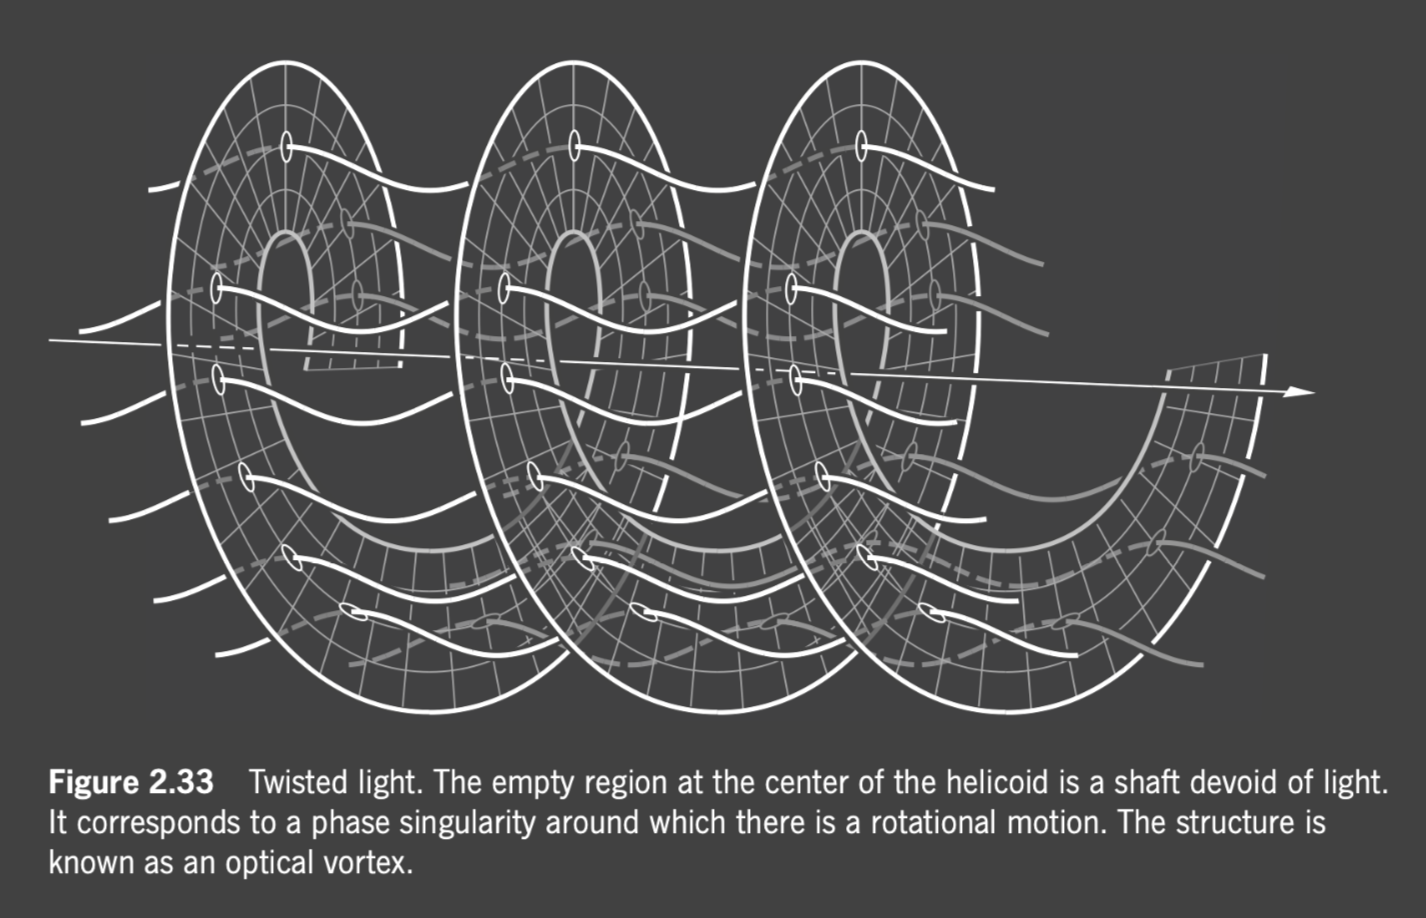
\includegraphics[width=0.6\textwidth]{Image/1_twisted_wave.png}
    \caption{Visualization of twisted light}
    \label{twisted_wave}
\end{figure}

\section*{各向异性介质中的波}
至今我们讨论的波相速度都没有\textbf{空间依赖性},而各向异性的介质会让波动方程的解析解几乎不可能得到。不过,有两条定律可以大大简化我们的分析:
\begin{theorem}[惠更斯原理 Huygens’ construction]
    给定一时刻的波前,其后的波前可以由每一点波动的波前的包络得到。
\end{theorem}
\begin{theorem}[费马原理 Fermat’s Principle]
    光总以最短距离到达。
\end{theorem}
根据惠更斯原理不难得到斯涅尔定律:
\begin{theorem}[斯涅尔折射定律 Snell's Refraction Law]
    \begin{equation}
        n_1\sin{\theta_1}=n_2\sin{\theta_2}
    \end{equation}
\end{theorem}
\indent 惠更斯原理在研究反射和折射现象的几何路径时候非常好用。据此可分析海市蜃楼的现象。
费马原理则需要考虑波的干涉。考虑从A到B的\textbf{光学路径(optical path)}:
\begin{equation}
    \bar{AB}=\int n(s)ds
\end{equation}
其中引入折射率来描述不同介质的速度差异。注意到大部分路径的波相位抵消,只有最短路径和最长路径的路径周围路径都相差相同相位而叠加增大。用该原理可以简洁地解释透镜的抛物线形状(令从物体出发到像的光学路径相等)。这两个定律在我们即将研究的几何光学中也非常有用。


\end{document}